\thispagestyle{quantoannone}
\pagestyle{quantoan}
\everymath{\color{quantoan}}
\graphicspath{{../quantoan/pic/}}
\blfootnote{\color{quantoan}\color{quantoan}$^1$Theo https://www.askamathematician.com/2009/12/q-do-you-exactly-know-what-einstein-meant-by-do-not-worry-about-your-difficulties-in-mathematics-i-can-assure-you-mine-are-still-greater/}
\begingroup
\AddToShipoutPicture*{\put(0,616){\includegraphics[width=19.3cm]{../bannerquantoan}}}
\AddToShipoutPicture*{\put(110,522){\includegraphics[scale=1]{../tieude.pdf}}}
\centering
\endgroup
\vspace*{185pt}

\begin{multicols}{2}
	
	\vspace*{-8pt}
	\PIbox{\textit{Đừng lo lắng về những khó khăn của các bạn trong toán học. Tôi có thể đảm bảo với các bạn  rằng tôi còn chật vật với toán hơn các bạn rất nhiều.}
		\vskip 0.01cm
		\hfill Albert Einstein}
	\vskip 0.2cm	
	Chúng ta sẽ cùng nghe ý kiến của một nhà toán học và của hai nhà vật lý bàn luận về câu nói này của Albert Einstein.
	\begin{figure}[H]
		\vspace*{-5pt}
		\centering
		\captionsetup{labelformat= empty, justification=centering}
		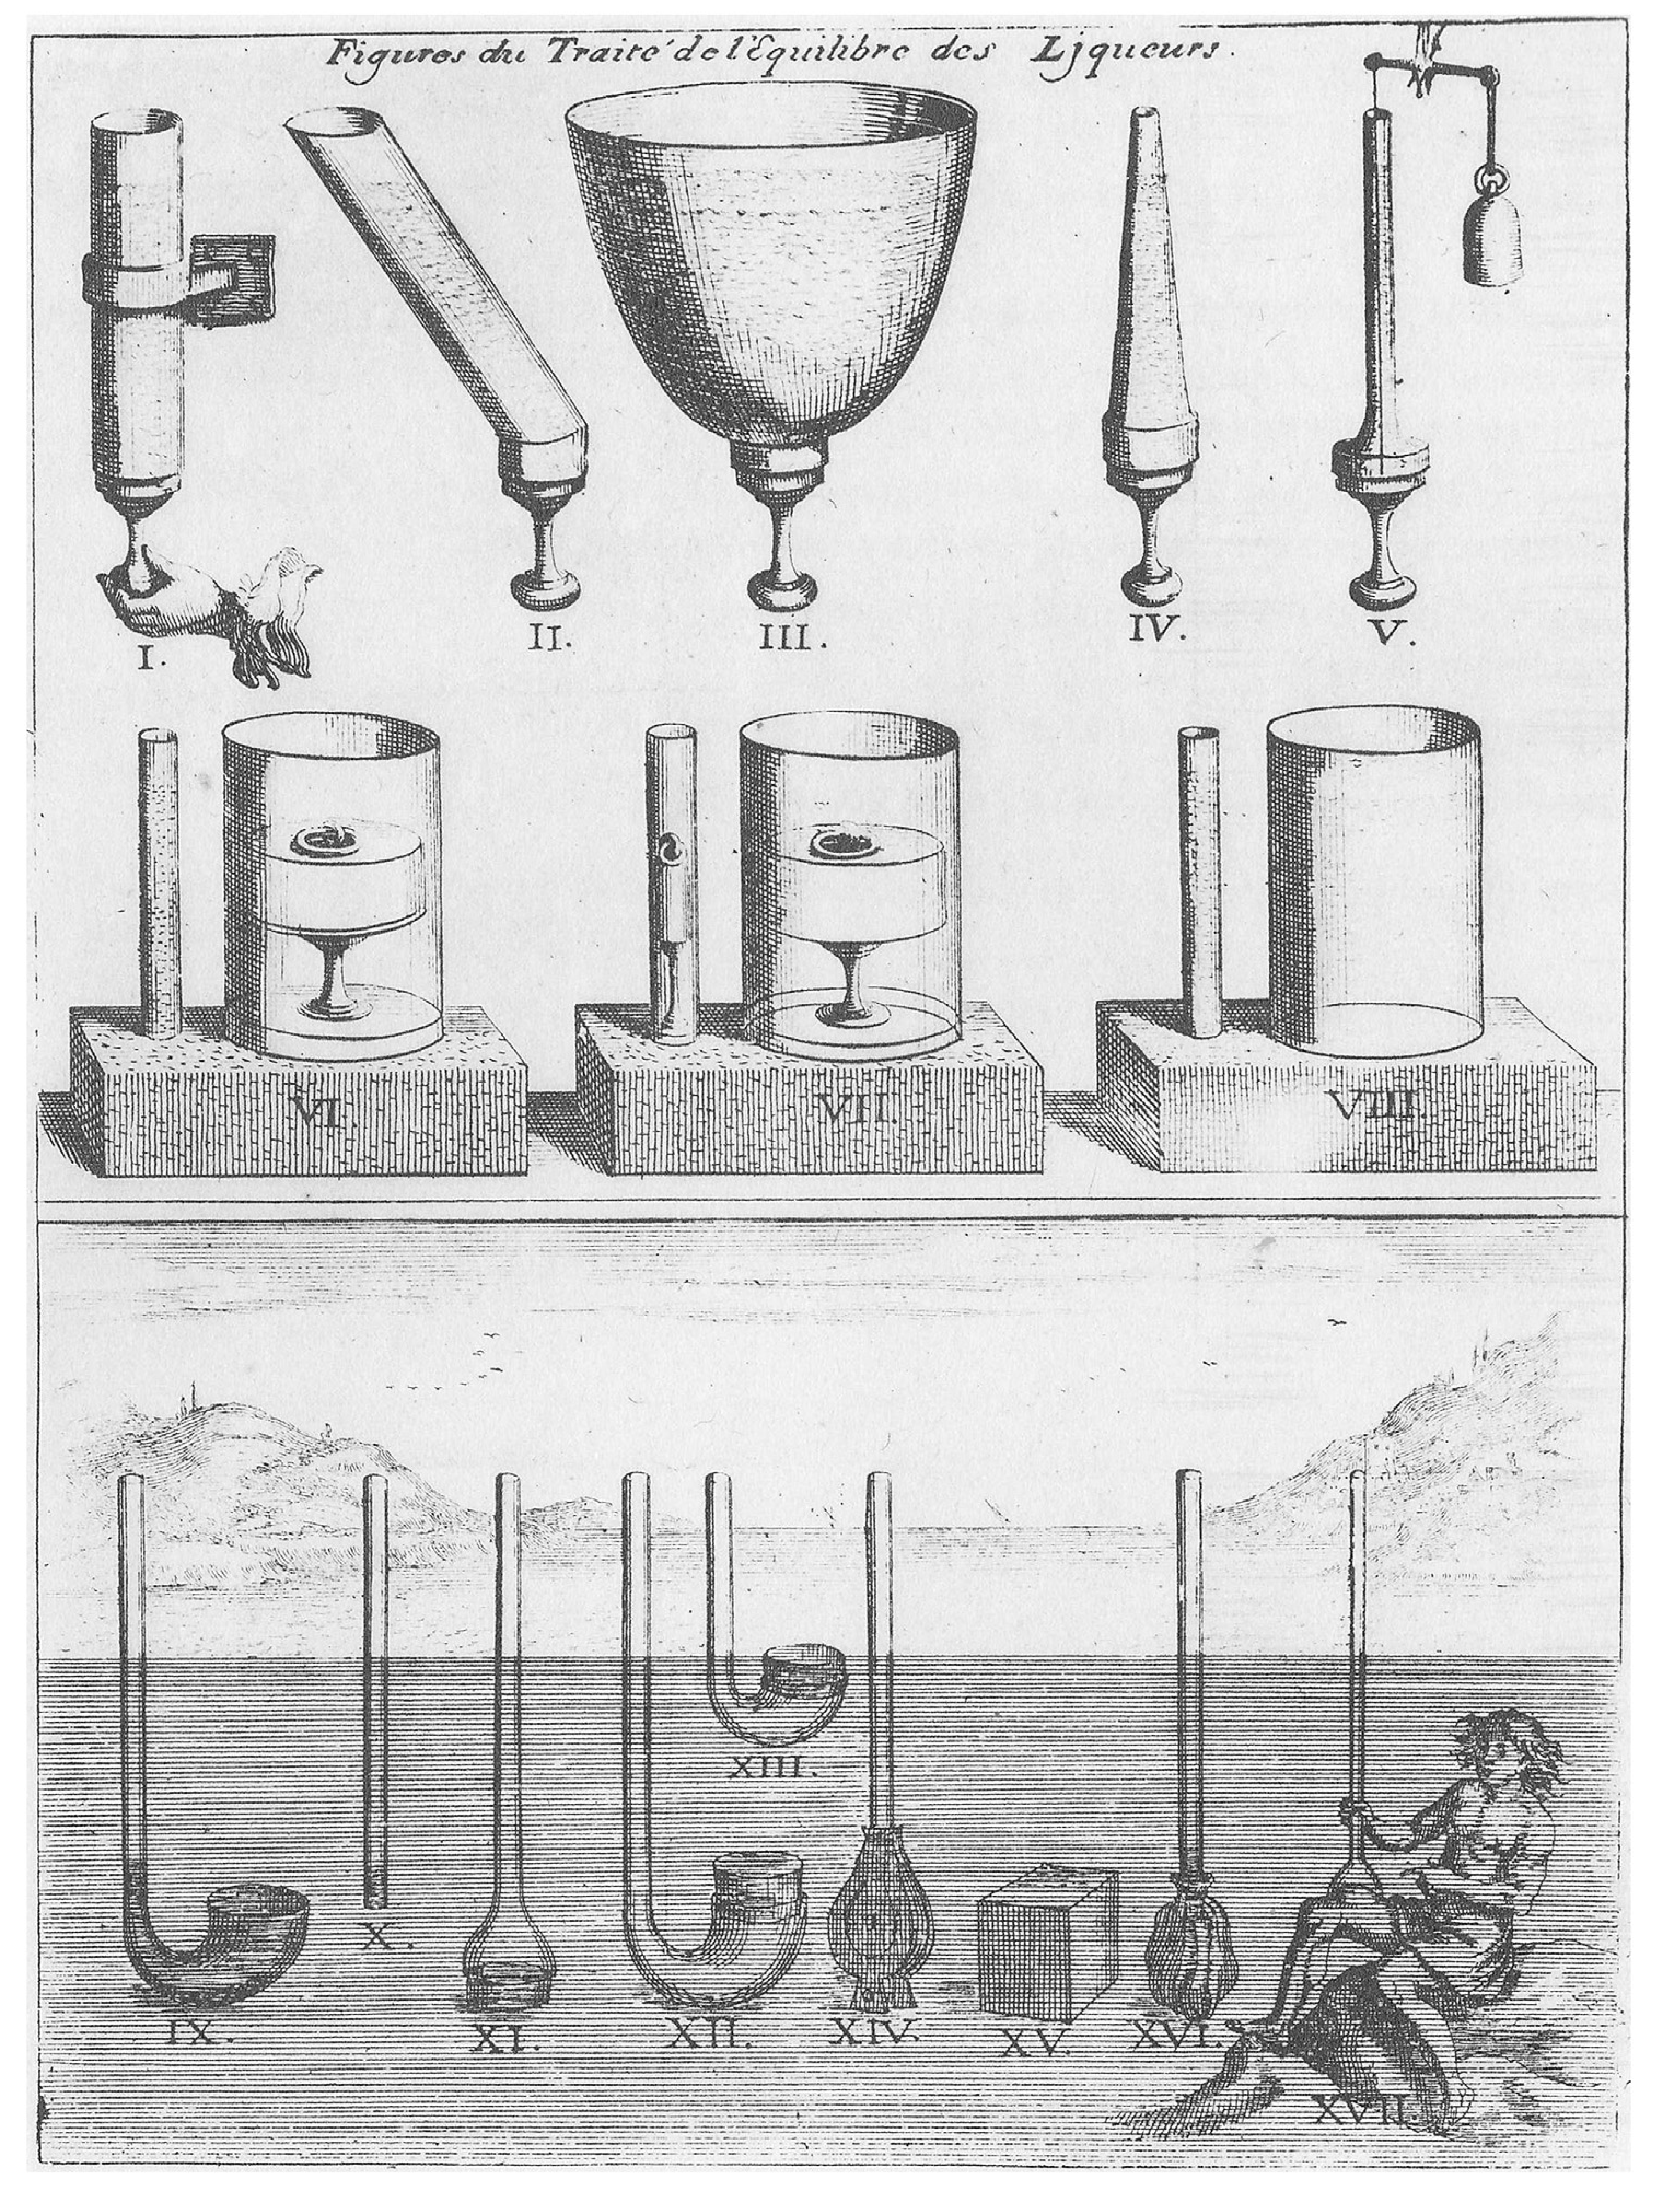
\includegraphics[width= 1\linewidth]{2}
		\caption{\small\textit{\color{quantoan}Minh họa Einstein bởi Laurent Taudin theo phong cách của Albert Uderzo.}}
		\vspace*{-10pt}
	\end{figure}
	\textbf{\color{quantoan}Nhà toán học:} Không thể biết chính xác ý của Einstein qua câu nói này nếu không hỏi ông ấy trực tiếp. Người ta thường cho rằng Einstein không hiểu sâu sắc về toán hoặc khi còn trẻ ông ấy học toán khá kém. Tuy nhiên, thật là lầm lẫn khi nói rằng Einstein kém về môn toán. Một số bài báo của ông khá phức tạp về mặt toán học, liên quan đến các môn học cao cấp như phương trình vi phân ngẫu nhiên và giải tích tensor. Hơn nữa, Einstein học toán rất xuất sắc khi còn trẻ.
	\vskip 0.1cm
	Có lẽ ý của Einstein khi tuyên bố gặp khó khăn trong môn toán là ông cảm thấy như thể phải vật lộn để học một số kiến thức toán rất cao cấp cần thiết cho việc phát biểu các lý thuyết của mình, hoặc rằng (so với các nhà toán học hoặc nhà vật lý toán học) kỹ năng toán học của ông không hoàn toàn được coi là mẫu mực. Tuy nhiên, chắc chắn Einstein có năng khiếu toán học bẩm sinh vượt hơn rất nhiều so với những người bình thường quanh bạn. Vì vậy, ta có thể luận ra được rằng câu trích dẫn ban đầu thực sự hướng đến các sinh viên trẻ tuổi, vì vậy nó chẳng qua  có thể chỉ phản ánh một nỗ lực nhằm  khuyến khích các sinh viên trẻ luôn kiên trì bất chấp những khó khăn mà họ cảm thấy được.
	\vskip 0.1cm
	\textbf{\color{quantoan}Nhà vật lý:} Đây là phỏng đoán của tôi. Einstein đã chứng kiến sự kết thúc của những gì có thể được coi là ``vật lý trực quan" của thế kỷ $19$ và trước đó. Điều này phần lớn là lỗi của chính ông. Vào năm $1905$ (``năm kỳ diệu" của Einstein), ông đã giới thiệu cho thế giới về cả \textit{cơ học lượng tử} và \textit{thuyết tương đối hẹp}. Cho đến thời điểm đó (hầu hết) vật lý hiện đại là thứ có thể dễ dàng hình dung và cảm nhận bằng trực giác. Bạn có thể vẽ các quỹ đạo của các vật thể di chuyển, điện trường và từ trường có thể được mô hình hóa bằng các đường, bạn có thể hình dung dòng nhiệt chảy như chất lỏng, v.v.
	\begin{figure}[H]
		\vspace*{-5pt}
		\centering
		\captionsetup{labelformat= empty, justification=centering}
		\includegraphics[width= 0.95\linewidth]{1}
		\caption{\small\textit{\color{quantoan}Các đường điện trường (màu xanh) có thể dễ dàng được thể hiện bằng hình vẽ trực quan.}}
		\vspace*{-10pt}
	\end{figure}
	Hơn nữa, thứ toán học được sử dụng trong đó khá đơn giản. Như kiểu toán đơn giản ta học ở  trường trung học. Với sự ra đời của thuyết tương đối và cơ học lượng tử, một thời đại của khoa học đã đến, ở đó những kết luận đạt được rơi tuột hoàn toàn ra khỏi sự kiểm soát của toán học truyền thống. Ngày nay, trực giác không chỉ trở thành hoàn toàn vô dụng, mà nó sẽ thường xuyên chủ động dẫn dắt bạn đi sai đường nhiều hơn là đi đúng hướng.
	\vskip 0.1cm
	Một số điều đầu tiên chúng ta học được về thuyết tương đối và cơ học lượng tử là: không có  khái niệm ``hiện tại" đối với hai điểm khác nhau, các hạt thực sự là các sóng, những sóng đó lại thực sự là các hạt, đi nhanh làm cho thời gian chậm lại, đi nhanh làm cho độ dài ngắn đi, năng lượng và vật chất chẳng qua là một, không gian và thời gian gần như giống nhau, đôi khi một số thứ sẽ đột nhiên xuất hiện ở phía bên kia của các rào cản mà chúng không thể vượt qua,  v.v.
	\vskip 0.1cm
	Không có thứ gì trong số các khái niệm này có thể được dự đoán bằng trực giác, và nhiều thứ trong số đó là kết quả của một số kiến thức và phép toán khá phức tạp.  Một nhánh của vật lý được nghiên cứu hiện nay (Mô hình chuẩn, Lý thuyết dây, và những thứ khác) sử dụng thứ toán học khó đến mức bạn phải mất nhiều năm bồi dưỡng về toán trước khi  có thể bắt đầu nắm bắt những gì đang xảy ra.  Einstein đã có nhiều năm được đào tạo về toán, nhưng có lẽ sẽ không thể tưởng tượng được sự đa dạng rộng lớn của các loại toán học khác nhau cần được vận dụng vì lý thuyết của ông.
	\vskip 0.1cm
	Chính bước nhảy vọt cuối cùng này về độ phức tạp trong toán  đã quật ngã Einstein.  Cậu bé  Einstein yêu quý của chúng ta  thực sự thông minh, thực sự giỏi toán trong trường phổ thông và là một người biết ăn mặc thời trang tinh tế.  Tuy nhiên, ngay cả những người mà bạn cho là thông minh  một cách không thể tưởng tượng được (tôi đang muốn nói về gốc họ Do Thái `Stein ở đây) hầu như sẽ luôn luôn bị che khuất bởi một người thông minh hơn và với sự chuẩn bị tốt hơn, chuyên sâu hơn.  Mặc dù Einstein có một nền tảng vật lý vững chắc, nhưng  phải cần tới các nhà toán học (với kiến thức toán và  gọng kính dày cộp của họ) mới có thể  đưa môn khoa học này tiến lên phía trước.
	\vskip 0.1cm
	\textbf{\color{quantoan}Ý kiến của một nhà vật lý khác:} Tôi không được biết  tới trích dẫn này của Einstein. Tôi chỉ có một phỏng đoán sơ bộ như sau. Trong khoảng thời gian từ khi công bố thuyết tương đối hẹp đến khi công bố  thuyết tương đối rộng, ông đã dành thời gian tìm hiểu hình học vi phân đủ để phát triển ý tưởng của mình. Đối với Einstein việc này hiển nhiên không hề dễ dàng  và cần rất nhiều tư vấn với những người khác ở Châu Âu. Chẳng hạn, Einstein và Levi--Civita thường xuyên liên lạc với nhau. Vì vậy, ông ấy có thể đã trả lời nhận xét của ai đó giống như khi chúng ta  nghe  thấy rằng bạn bè của ta đang có một thời gian khó khăn với môn toán.
	\vskip 0.1cm
	\textbf{\color{quantoan}Bản thân Einstein và những người đương thời nói gì?}
	\vskip 0.1cm
	Câu trích dẫn sau đây của Einstein có thể giúp chúng ta có thêm một góc nhìn:
	\vskip 0.1cm
	``Từ khi các nhà toán học đổ bộ vào thuyết tương đối, tôi không còn hiểu được nó nữa."
	\vskip 0.1cm
	\hfill (A. Sommerfelt 
	\vskip 0.01cm
	\hfill``\textit{To Albert Einstein's Seventieth Birthday}")
	\vskip 0.1cm
	Có khả năng Einstein đã nói điều này vào một lúc nào đó khoảng giữa năm $1907$ (khi Minkowski giảng bài về cách phát biểu lại thuyết tương đối hẹp) và năm $1912$ (khi Einstein nhận ra rằng ông cần một cách tiếp cận hình học để xây dựng thuyết tương đối rộng).
	\vskip 0.1cm
	Các nhận xét khác cũng được lưu lại trong khoảng thời gian này bao gồm nhận xét của Einstein trong một bài giảng, khi ông cần rút ra một kết quả cụ thể:
	\vskip 0.1cm
	``Điều này đã được thực hiện một cách tao nhã bởi Minkowski; nhưng viên phấn thì rẻ hơn chất xám, và chúng ta sẽ làm điều đó một cách tuỳ biến mà không gò bó."
	\vskip 0.1cm
	\hfill(thuật lại bởi Polya trong cuốn
	\vskip 0.01cm
	\hfill \textit{Littlewood's Miscellany})
	\vskip 0.1cm
	Sau đó, Einstein nhận ra rằng thuyết tương đối rộng có thể không chỉ yêu cầu những khái niệm này mà còn cần những mở rộng cao cấp hơn của những khái niệm đó:
	\vskip 0.1cm
	``Vấn đề này vẫn không giải quyết được đối với tôi cho đến năm $1912$, khi tôi đột nhiên nhận ra rằng lý thuyết mặt của Gauss nắm giữ chìa khóa để giải mã bí ẩn này. Tôi nhận ra rằng tọa độ bề mặt của Gauss có một ý nghĩa sâu sắc. Tuy nhiên, lúc đó tôi không biết rằng Riemann đã nghiên cứu cơ sở của hình học một cách sâu sắc hơn nữa. Tôi chợt nhớ rằng lý thuyết của Gauss có trong khóa học hình học do Geiser đưa ra khi tôi còn là sinh viên...
	\vskip 0.1cm
	Tôi nhận ra rằng nền tảng của hình học có ý nghĩa vật lý. Người bạn thân của tôi, nhà toán học Grossmann đã ở đó khi tôi từ Praha trở về Zurich. Từ ông ấy, lần đầu tiên tôi biết về Ricci và sau đó là Riemann. Vì vậy, tôi đã hỏi bạn tôi rằng liệu vấn đề của tôi có thể được giải quyết bằng lý thuyết Riemann hay không, cụ thể là liệu các bất biến của yếu tố đường có thể xác định hoàn toàn các đại lượng mà tôi đang tìm kiếm hay không."
	\vskip 0.1cm
	\hfill (Einstein, \textit{Bài giảng Kyoto}, $1922$)
	\vskip 0.1cm
	Sau khi đã tạo ra được những sự liên hệ này vào năm $1912$, Einstein không còn lựa chọn nào khác ngoài việc học hình học cao cấp mà ông còn thiếu -- chủ yếu là từ Grossmann. Khi  đã  thực hiện được như vậy, ông có thể sử dụng hình học cao cấp để phát biểu thuyết tương đối rộng.
	\vskip 0.1cm
	Sau này, David Hilbert có tâm sự với người viết tiểu sử của mình:
	\vskip 0.1cm
	``Mọi cậu học trò trên những con phố của thủ đô toán học này [Göttingen] đều hiểu về hình học bốn chiều tốt hơn Einstein. Tuy nhiên, bất chấp điều này, Einstein đã làm được việc, chứ không phải các nhà toán học."
	\vskip 0.1cm
	\hfill (Constance Reid, \textit{Hilbert}, Springer,  $1996$)
	\vskip 0.1cm
	Đây quả là một tuyên bố hào phóng của Hilbert, vì ông đã suýt đánh bại được Einstein trong cuộc chạy đua cuối cùng đến các phương trình trường của thuyết tương đối rộng. Nhưng ông nhận ra rằng tài năng vật lý của Einstein đã cho phép ông ấy làm được nhiều thứ hơn việc bù đắp những sự thiếu hụt của mình về các tinh tế toán học.
	\vskip 0.1cm
	\textbf{\color{quantoan}Tài liệu tham khảo}
	\vskip 0.1cm
	[$1$]	Constance Reid, \textit{Hilbert}, Springer,  $1996$.
	\vskip 0.1cm
	[$2$]	A. Sommerfelt ``\textit{To Albert Einstein's Seventieth Birthday}" in Paul A. Schilpp (ed.) \textit{Albert Einstein}, Philosopher--Scientist, Evanston, $1949$.
	\vskip 0.1cm
	[$3$] Littlewood, J. E. $(1986)$, Bollobás, Béla (ed.), \textit{Littlewood's miscellany}, Cambridge: Cambridge University Press.
\end{multicols}